\listfiles
\documentclass[11pt,a4paper]{article}

\title{\titolo}
\author{\autorea \and \autoreb \and \autorec}
\date{\today}

\usepackage{preambolo,lipsum}

\begin{document}\maketitle
\begin{abstract}
  \noindent In questo articolo vengono brevemente presentati il
  programma \emacs{} ed il pacchetto \auctex{} per le principali
  piattaforme: Windows, GNU/Linux e Mac OS. Dopo una introduzione ai
  programmi, verranno esposte le modalità per poter installare e
  configurare \emacs{} e \auctex{} per poter scrivere documenti
  \LaTeX{}. L'articolo non ha la pretesa di essere un \emph{manuale},
  bensì un piccolo tutorial per far avvicinare gli utenti di \LaTeX{}
  a questo programma, non così troppo complicato come spesso viene
  indicato.
\end{abstract}

\begin{multicols}{2}
  \tableofcontents
\end{multicols}

\section{Introduzione}
\label{sec:intro}

\textcolor{red}{\lipsum[1]}

Lo sviluppo di \emacs{} è iniziato negli anni 1970 ai laboratori di Intelligenza
Artificiale del MIT, cioè molto prima che si diffondesse l'informatica che
conosciamo oggi.  Ciò comporta che \emacs{} utilizza una terminologia spesso
diversa da quella utilizzata dalla stragrande maggioranza degli altri programmi
che usiamo quotidianamente.  Per questo motivo non bisogna sorprendersi se
l'operazione di \emph{tagliare} del testo (generalmente indicata in inglese con
\emph{cutting}) in \emacs{} viene chiamata \emph{killing} e la successiva
operazione di \emph{incollare} il testo copiato (in inglese \emph{pasting})
viene chiamata \emph{yanking}.

\emacs{} è famoso per rendere possibile l'esecuzione di qualsiasi operazione
usando solo la tastiera, cioè senza l'ausilio del mouse.  A ogni comando può
essere associata una combinazione di tasti.  In questa guida seguiremo la
notazione diffusa nel mondo di \emacs{} per indicare i tasti.  Quindi il tasto
\verb!Control! verrà indicato con \verb!C!, l'\verb!Invio! viene indicato con
\verb!RET!, mentre \verb!M! indica il tasto \verb!Meta!.  Sulle odierne tastiere
questo tasto è scomparso, si può ottenere lo stesso risultato con il tasto
\verb!Alt! oppure premendo e rilasciando il tasto \verb!Esc!.  Un trattino fra
due tasti all'interno di una combinazione di tasti indica che i tasti vanno
premuti contemporaneamente.  Così, quando si dirà che per eseguire un comando
bisogna usare la combinazione \verb!M-x! si dovranno premere contemporaneamente
il tasto \verb!Alt! e la lettera \verb!x! oppure premere il tasto \verb!Esc!,
rilasciarlo e premere la lettera \verb!x!.

Il manuale di \emacs{} può essere consultato all'interno dello stesso editor di
testo con le combinazioni di tasti \verb!C-h r! (premere contemporaneamente il
tasto \verb!Control! e la lettera \verb!h!, rilasciare questi tasti e premere la
lettera \verb!r!) oppure \verb!C-h i d m Emacs RET! (premere contemporaneamente
il tasto \verb!Control! e la lettera \verb!h!, rilasciare questi tasti e premere
la lettera \verb!i!, poi la lettera \verb!d!, poi la lettera \verb!m!, poi
scrivere \verb!Emacs! quindi premere il tasto \verb!Invio!).  Se si preferisce,
il manuale può anche essere consultato dal menu
\begin{Verbatim}
Help > Read the Emacs Manual
\end{Verbatim}


\section{Installare \emacs}
\label{sec:install}

\subsection{\emacs{} per Windows}
\label{sec:installwin}


Per sistemi operativi Microsoft Windows non esiste una vera e propria
procedura di installazione. \emacs{} si può utilizzare semplicemente
procurandosi l'archivio che contiene gli eseguibili.

Dal sito ufficiale di \emacs{} per Windows %
\sito{http://ftp.gnu.org/pub/gnu/emacs/windows/}{\emacs\ for Windows} %
si scarica l'archivio compresso %
\href{http://ftp.gnu.org/pub/gnu/emacs/windows/emacs-23.4-barebin-i386.zip}
{\textsf{emacs-23.4-barebin-i386.zip}} e lo si decomprime in una
posizione di comodo; una buona soluzione, per esempio, è decomprimere
il suddetto archivio in:
\begin{Verbatim}
C:/Programmi/emacs/
\end{Verbatim}

Se si vuole creare un collegamento di \emacs{} nel menù Start, è
sufficiente un doppio clic sul file \emph{addpm.exe} contenuto nella
cartella:
\begin{Verbatim}
C:/Programmi/emacs/bin
\end{Verbatim}

\subsection{\emacs{} per GNU/Linux}
\label{sec:installlinux}


\emacs{} fa parte del progetto GNU quindi è presente in tutti i
sistemi operativi della famiglia GNU/Linux. Se non è già installato,
il metodo più semplice per ottenere \emacs{} in un sistema GNU/Linux è
far riferimento al gestore pacchetti della propria distribuzione. Si
possono naturalmente utilizzare i gestori di pacchetti a interfaccia
grafica, riportiamo qui inoltre i comandi da terminale che possono
essere eseguiti per installare \emacs{} in alcune delle principali
distribuzioni: Debian e Ubuntu:
\begin{Verbatim}
$ sudo apt-get install emacs
\end{Verbatim}
% $
Fedora:
\begin{Verbatim}
$ sudo yum install emacs
\end{Verbatim}
% $
OpenSUSE:
\begin{Verbatim}
$ sudo zypper install emacs
\end{Verbatim}
% $

Il metodo più difficile, per i non avvezzi all'uso del terminale,
consiste nel compilare \emacs{} a partire dal codice sorgente,
tuttavia non è intenzione di questa guida spiegare come fare ciò.

Dopo averlo installato, \emacs{} potrà essere avviato facendo clic sul
suo lanciatore oppure eseguendo da terminale il comando
\begin{Verbatim}
$ emacs
\end{Verbatim}
% $
Se si desidera utilizzare \emacs{} con interfaccia testuale bisogna
aggiungere l'opzione \texttt{-nw} oppure \texttt{--no-window-system}:
\begin{Verbatim}
$ emacs -nw
\end{Verbatim}
% $
Possono essere aggiunti come argomenti da linea di comando il percorso
del file (o dei file) che si vogliono modificare:
\begin{Verbatim}
$ emacs file1.tex file2.tex
\end{Verbatim}
% $

\subsection{\emacs{} per Mac OS}

Sul mirror ufficiale %
\sito{http://ftp.gnu.org/pub/gnu/emacs/windows/}{\emacs} non
è presente una versione già compilata per Mac OS X, queste versioni
sono rese disponibili da vari volontari come ad esempio il gestore del
sito \sito{http://emacsformacosx.com/}{Emacs for Mac OS X}. La
procedura per l'installazione è quella consueta: scaricata la versione
più recente si apre il file dmg (se non è già stato aperto
automaticamente al termine del download) e si trascina Emacs nella
cartella Applicazioni.

In Mac OS le applicazioni avviate dall'interfaccia grafica non hanno
accesso ai valori delle variabili d'ambiente, per rendere disponibile
ad \emacs{} la variabile \texttt{PATH} è necessario dare da terminale
il comando
\begin{Verbatim}
$ defaults write ~/.MacOSX/environment PATH "$PATH"
\end{Verbatim}
Le nuove impostazioni sono effettive dopo aver eseguito un logout e un
successivo login.

Il comando va ripetuto ogni volta che si installa qualche programma
che modifica il valore di \texttt{PATH}, il caso che più probabilmente
riguarda i lettori di questa guida è la distribuzione \TeX{}.

Per gli utenti che usano la tastiera italiana è utile impostare il
tasto \texttt{cmd} come \texttt{meta} e il tasto \texttt{alt} per
scrivere i caratteri speciali, in particolare le parentesi quadre, le
graffe e la tilde, scrivendo queste righe nel file \emph{.emacs}
\begin{Verbatim}
(setq ns-command-modifier 'meta)
(setq ns-alternate-modifier nil)
\end{Verbatim}

\section{Installare \auctex}
\label{sec:installauc}

\subsection{\auctex{} per Windows}
\label{sec:auctexwin}

Dal sito ufficiale di \auctex{} per Windows %
\sito{http://www.gnu.org/software/auctex/download-for-windows.html}%
{\auctex\ For Windows}, %
si scarica l'archivio compresso %
\href{http://ftp.gnu.org/pub/gnu/auctex/auctex-11.86-e23.2-msw.zip}%
{\textsf{auctex-11.86-e23.2-msw.zip}} e lo si decomprime in
\begin{Verbatim}
C:/Programmi/emacs/
\end{Verbatim}
Sia nell'archivio di \auctex{}, che quello di \emacs, posizionato in precedenza
nel percorso suddetto, vi è una cartella dal nome \emph{site-lisp}: i file
contenuti in queste cartelle vanno uniti in una sola cartella.

\subsection{\auctex{} per GNU/Linux}
\label{sec:auctexlinux}

Anche il pacchetto \auctex{} è presente nei sistemi GNU/Linux. Come già detto
per \emacs, per installare \auctex{} si consiglia di utilizzare il gestore
pacchetti della propria distribuzione. Ecco i comandi da usare per installare da
terminale il pacchetto nelle principali distribuzioni: Debian e Ubuntu:
\begin{Verbatim}
$ sudo apt-get install auctex
\end{Verbatim}
% $
Fedora:
\begin{Verbatim}
$ sudo yum install emacs-auctex
\end{Verbatim}
% $
OpenSUSE:
\begin{Verbatim}
$ sudo zypper install emacs-auctex
\end{Verbatim}
% $


\subsection{\auctex{} per Mac OS}
\label{sec:auctexmac}

Come per \emacs{} non è disponibile una versione di \auctex{} già compilata per
Mac OS, in questo caso non esistono neppure versioni non ufficiali ed è quindi
necessario utilizzare l'utility \texttt{make}.  \texttt{make} viene installato
insieme all'ambiente di sviluppo
\href{http://developer.apple.com/technologies/tools/whats-new.html}%
{Xcode}, chi non intende dedicare svariati GB di disco a un software utile
soltanto a chi sviluppa software può sfuttare il fatto che \texttt{make} viene
installato anche dal correttore ortografico
\href{http://cocoaspell.leuski.net/}{cocoaspell} la cui installazione è
descritta nel paragrafo \ref{sec:aspellmac}.

Dalla pagina relativa a Mac OS
\sito{http://www.gnu.org/software/auctex/download-for-macosx.html}%
{\auctex\ For Mac OS X} bisogna scaricare l'archivio
\href{http://ftp.gnu.org/pub/gnu/auctex/auctex-11.86.tar.gz}%
{auctex-11.86.tar.gz}.

Dopo aver estratto il contenuto dell'archivio in una cartella temporanea occorre
aprire una sessione di terminale e portarsi nella cartella appena creata.

Configurare \auctex{} con il comando
\begin{Verbatim}
$ ./configure --prefix=/Applications/Emacs.app/Contents/Resources/\
  --with-emacs=/Applications/Emacs.app/Contents/MacOS/Emacs\
  --with-lispdir=/Applications/Emacs.app/Contents/Resources/site-lisp/\
  --without-texmf-dir
\end{Verbatim}
% $
sostituendo se necessario a \texttt{Applications}\footnote{Utilizzando il
  terminale non bisogna utilizzare i nomi localizzati delle cartelle ma quelli
  reali, quindi \texttt{Application} è corretto anche se si utilizza la versione
  italiana di Mac OS} la cartella in cui si trova Emacs, in questo modo tutti i
file saranno contenuti nel bundle \texttt{Emacs.app}.

Compilare e installare con il comando
\begin{Verbatim}
$ make && make install
\end{Verbatim}
%$

Dopo l'installazione bisogna impostare i visualizzatori per i vari file creati
con \LaTeX{} scrivendo nel file \emph{.emacs} queste righe
\begin{Verbatim}
(setq TeX-view-program-list
      '(("dvips and Skim" "%(o?)dvips %d -o &&\
  /Applications/Skim.app/Contents/SharedSupport/displayline %n %f %b")
         ("Skim" "/Applications/Skim.app/Contents/SharedSupport/\
displayline %n %o %b")
        ("open" "open %o")))
(setq TeX-view-program-selection
      '(((output-dvi style-pstricks) "dvips and Skim")
        (output-dvi "Skim")
        (output-pdf "Skim")
        (output-html "open")))
\end{Verbatim}
Come visualizzatore principale si utilizza
\href{http://skim-app.sourceforge.net/}{Skim} perché supporta la ricerca diretta
e inversa dal pdf, i dettagli sulla configurazione di \emacs{} e Skim sono
riportati nel paragrafo \ref{sec:fismac}.

\section{Personalizzare \emacs{} \& \auctex} % titolo cambiato per avere un
% effetto migliore nell'indice, ma in realtà non mi piace
\label{sec:personal}

Una delle caratteristiche principali di \emacs{} è che è un editor di testo
personalizzabile in ogni suo aspetto ed espandibile, in modo da renderlo adatto
alle proprie esigenze.  In questo paragrafo vedremo alcune delle
personalizzazioni che possono risultare utili quando si lavora con documenti
\LaTeX{}.  Il linguaggio utilizzato per espandere \emacs{} è l'Elisp, un
dialetto del Lisp sviluppato appositamente per \emacs{}.

Per modificare le impostazioni relative alla gestione nativa di \TeX{} da parte
di \emacs{} è possibile usare la funzione
\verb!M-x customize-group RET tex RET!.  In questo modo si aprirà un buffer nel quale sarà possibile modificare,
tramite l'interfaccia, le opzioni desiderate.  Per modificare in particolare
\auctex{} è possibile usare la funzione
\verb!M-x customize-group RET AUCTeX RET!.

Di seguito saranno suggerite alcune porzioni di codice Elisp che permettono di
personalizzare \emacs{} e che vanno inserite nel file di inizializzazione
\verb!~/.emacs!.  Per rendere effettive le modifiche bisogna riavviare \emacs{}.

Se si usa \auctex{}, è possibile inserire macro nei propri documenti \LaTeX{}
con \verb!C-c RET!.  La comodità di questa funzione è che \auctex{} conosce le
macro dei principali pacchetti \LaTeX{} e permette quindi l'autocompletamento
con il tasto TAB.  Inoltre conosce gli argomenti e le opzioni che queste macro
accettano, infatti usando \verb!C-c RET frac RET! nel documento si otterrà
\verb!\frac{}{}!  e il cursore si posizionerà all'interno del primo paio di
parentesi graffe.  Allo stesso modo, usando \verb!C-c RET sqrt RET! verrà
richiesto l'ordine \verb!n! della radice da inserire (premere direttamente
\verb!RET! per non inserire nulla) e si otterrà \verb!\sqrt[n]{}!.  Per fare in
modo che \auctex{} conosca quali pacchetti \LaTeX{} sono stati caricati bisogna
permettergli di effettuare il parsing dei propri documenti e questo è possibile
aggiungendo nel proprio file \verb!.emacs! il seguente codice
\begin{Verbatim}
(setq TeX-parse-self t) ; Attiva parsing al caricamento.
(setq TeX-auto-save  t) ; Attiva parsing al salvataggio.
\end{Verbatim}
In questo modo verrà creata una cartella chiamata \verb!auto! nella stessa
directory in cui si trova il documento nella quale verranno registrate le
informazioni relative al proprio documento \LaTeX{}, se non si desidera
affollamento nelle proprie cartelle si potrebbe non voler attivare queste due
opzioni.

Come detto, \auctex{} conosce le macro dei pacchetti principali, ma naturalmente
non conosce tutte i pacchetti.  Possiamo, però, fargli conoscere delle macro
aggiuntive da utilizzare solo quando viene caricato nel documento \LaTeX{} il
pacchetto che fornisce le relative macro.  Per esempio, \auctex{} non conosce le
macro messe a disposizione dal pacchetto \verb!siunitx!.  Con il seguente codice
da aggiungere nel file \verb!.emacs! apprenderà che questo pacchetto fornisce i
comandi \verb!SI!, \verb!si! e \verb!num! di cui il primo accetta due argomenti,
gli ultimi due solo uno:
\begin{Verbatim}
(eval-after-load "tex"
  '(TeX-add-style-hook
    "siunitx"
    (lambda ()
      (TeX-add-symbols
       '("SI" 2)
       '("si" 1)
       '("num" 1)))))
\end{Verbatim}
A volte in un documento \LaTeX{} non si carica un certo pacchetto \verb!A!
poiché è automaticamente caricato da un altro pacchetto \verb!B! che viene
esplicitamente caricato.  In questi casi, però, \auctex{} potrebbe non rendersi
conto che il pacchetto \verb!A! è stato effettivamente caricato e non fornirebbe
le funzioni di autocompletamento per le macro del pacchetto \verb!A!, se è uno
di quelli supportati.  Per ovviare a questo problema è possibile inserire il
seguente codice nel file di inizializzazione
\begin{Verbatim}
(eval-after-load "tex"
  '(TeX-add-style-hook
    "B"
    (lambda ()
      (TeX-run-style-hooks "B"))))
\end{Verbatim}
Per esempio, il pacchetto \verb!kpfonts! carica automaticamente il pacchetto
\verb!amsmath! e non è quindi necessario inserire nel proprio sorgente \LaTeX{}
l'istruzione \verb!\usepackage{amsmath}!.  Per far sapere ad \auctex{} questa
situazione si userà il codice
\begin{Verbatim}
(eval-after-load "tex"
  '(TeX-add-style-hook
    "kpfonts"
    (lambda ()
      (TeX-run-style-hooks "amsmath"))))
\end{Verbatim}

Se si è soliti suddividere i propri documenti \LaTeX{} in più file da includere
nel file principale con i comandi \verb!\input! o \verb!\include! può essere
utile aggiungere al file \verb!.emacs!
\begin{Verbatim}
(setq-default TeX-master nil)
\end{Verbatim}
In questo modo, all'apertura dei documenti \LaTeX{} \emacs{} chiederà qual è il
file principale associato e sul quale saranno eseguiti i comandi di
compilazione.

Se si usa spesso \LaTeX{} per comporre documenti matematici potrebbe essere
utile attivare la modalità \verb!LaTeX-math-mode! con \verb!C-c ~! oppure con il
comando \verb!M-x LaTeX-math-mode!.  In questo modo, per esempio, per inserire
il simbolo \verb!\alpha! si potrà usare la scorciatoia \verb!` a!.  L'elenco
delle altre scorciatoie per inserire i simboli può essere consultato dal menu
\verb!Math! nella barra dei menu.  Per attivare automaticamente questa modalità
ogni volta che si apre un documento \LaTeX{} bisogna aggiungere
\begin{Verbatim}
(add-hook 'TeX-mode-hook 'LaTeX-math-mode)
\end{Verbatim}
al proprio \verb!.emacs!.

Il codice
\begin{Verbatim}
(setq TeX-electric-sub-and-superscript t)
\end{Verbatim}
aggiunto al proprio \verb!.emacs!, permette di inserire automaticamente una
coppia di parentesi graffe \verb!{}! quando si scrivono i simboli \verb!_! e
\verb!^! in modalità matematica.

Normalmente, quando si preme \verb!RET! in un sorgente \LaTeX{} viene
semplicemente aggiunta una nuova linea.  Se si vuole che andando a capo la nuova
linea sia automaticamente indentata bisogna premere \verb!C-j! invece di
\verb!RET!.  Si può però fare in modo che si ottenga questo risultato anche
premendo normalmente \verb!RET! aggiungendo il seguente codice al file di
inizializzazione
\begin{Verbatim}
(setq TeX-newline-function 'newline-and-indent)
\end{Verbatim}
Se si mette \verb!reindent-then-newline-and-indent! al posto di
\verb!newline-and-indent! si avrà, in più, l'effetto che la riga attuale viene
indentata.

\section{Correttore ortografico}
\label{sec:corr}

Per abilitare \emacs{} e \auctex{} a lavorare con la lingua italiana bisogna
installare il correttore ortografico. Le procedure, poiché differenti, vengono
di seguito esposte per tutti e tre i sistemi operativi.  L'uso, invece, è
invariante.

Per fare una revisione del documento che si sta scrivendo, bisogna premere la
combinazione di tasti \verb!M-x! e scrivere \verb!ispell!: in questo modo il
dizionario proporrà, in sequenza, la correzione dei termini che trova errati.

Un secondo modo, per scrivere correttamente, è attivare la modalità
\emph{flyspell} (correzione al volo). Se la si vuole attivare solo sul documento
corrente basta andare in \texttt{Tools > Spell Checking > Automatic spell
  checking (Flyspell)}; se invece la si vuole tenere sempre abilitata si deve
aggiungere la riga:
\begin{Verbatim}
(add-hook 'LaTeX-mode-hook 'flyspell-mode)
\end{Verbatim}
al proprio file \emph{.emacs}.

Quando viene rilevata una parola potenzialmente non corretta, questa verrà
colorata (in genere) in rosso. Alcuni termini, però, vengono segnalati come
errati anche quando sono corretti, cosa che accade perché quel termine non è
presente nel dizionario: si può aggiungerlo, premendo il tasto centrale del
mouse quando questo è posizionato sulla parola e scegliere \texttt{Save word}.

\subsection{Windows}
\label{sec:aspellwin}

Per usare il correttore ortografico in \emacs, su un sistema operativo Windows,
si può installare il programma GNU Aspell
\sito{http://aspell.net/win32/}{GNU Aspell - Win32 version}. L'ultima
versione stabile per Windows, seppur datata Dicembre 2002, è la 0.50-3.

I file che bisogna procurarsi sono quelli che vengono di seguito
riportati; si badi bene ad installarli nell'ordine in cui vengono
dati:

\begin{enumerate}
\item il programma completo
  \href{http://ftp.gnu.org/gnu/aspell/w32/Aspell-0-50-3-3-Setup.exe}%
  {Aspell-0-50-3-3-Setup.exe} (che rappresenta il programma
  vero e proprio);
\item il dizionario precompilato per l'italiano
  \href{http://ftp.gnu.org/gnu/aspell/w32/Aspell-it-0.50-2-3.exe}%
  {Aspell-it-0.50-2-3.exe}.
\end{enumerate}

Resta qualche altra operazione da fare. Come prima cosa si deve copiare il
percorso della cartella dove sono contenuti gli eseguibili di Aspell nella
variabile d'ambiente \textsf{PATH} di Windows. Secondo, aggiungere al proprio
\emph{.emacs} le seguenti righe di codice:
\begin{Verbatim}
(setq-default ispell-program-name "aspell")
(setq-default ispell-extra-args '("--reverse"))
(setq ispell-dictionary "italiano")
\end{Verbatim}
dove, la prima e la terza sono quelle strettamente necessarie, mentre la seconda
riga serve a risolvere dei problemi con le versioni precedenti di
\emacs. % SICURO??? CHIEDERE

\subsection{GNU/Linux}
\label{sec:aspelllinux}

Il correttore ortografico GNU Aspell può essere installato facilmente
su GNU/Linux utilizzando, come al solito, il gestore pacchetti della
propria distribuzione. Il dizionario italiano di GNU Aspell si chiama
\texttt{aspell-it} quindi da terminale può essere installato in Debian
con il comando
\begin{Verbatim}
$ sudo apt-get install aspell-it
\end{Verbatim}
% $
in Fedora con
\begin{Verbatim}
$ sudo yum install aspell-it
\end{Verbatim}
% $
mentre in openSUSE si può eseguire il comando:
\begin{Verbatim}
$ sudo zypper install aspell-it
\end{Verbatim}
% $

\subsection{Mac OS}
\label{sec:aspellmac}

Anche per Mac OS X è disponibile una versione di \textsf{GNU Aspell}
\sito{http://cocoaspell.leuski.net/}{cocoAspell}

Dopo aver installato \href{http://people.ict.usc.edu/~leuski/%
  cocoaspell/cocoAspell.2.1.dmg}{cocoAspell.2.1} si possono installare
i dizionari delle lingue che interessano scaricandoli direttamente dal
sito di (\href{ftp://ftp.gnu.org/gnu/aspell/dict/}{\textsf{GNU
    Aspell}}), ad esempio il dizionario italiano è contenuto
nell'archivio
\href{ftp://ftp.gnu.org/gnu/aspell/dict/it/aspell6-it-2.2_20050523-0.tar.bz2}%
{aspell6-it-2.2\_20050523-0.tar.bz2}.

Dopo aver scaricato i dizionari bisogna estarre il contento
dell'archivio in una cartella temporanea, aprire una sessione di
terminale e portarsi nella cartella appena creata. I dizionari si
installano dando i seguenti comandi
\begin{Verbatim}
$ ./configure
$ make
$ sudo make install
\end{Verbatim}
% $

Come ultima cosa è necessario configurare \emacs\ aggiungendo al
\emph{.emacs} le seguenti righe:
\begin{Verbatim}
(setq-default ispell-program-name "aspell")
(setq ispell-dictionary "italiano")
\end{Verbatim}

\section{Ricerca diretta-inversa}
\label{sec:ricdirinv}

Una delle principali funzioni che spesso gli utenti di \LaTeX{} cercano nel
proprio editor è quella della ricerca diretta-inversa, molto utile in fase di
revisione finale del proprio documento, e specie quando quest'ultimo è
abbastanza corposo.

Alcuni editor di testo hanno un visualizzatore integrato già configurato per
effettuare la ricerca dal file sorgente tex al documento pdf e viceversa, come
per esempio \TeX works, \TeX maker e qualche altro; altri, come \emacs,
richiedono alcuni passaggi per arrivare allo scopo.

Le procedure per usare tale funzione in \emacs{} variano per i tre sistemi
operativi citati in questa guida, quindi, come per le altre funzioni, saranno
descritte in altrettanti paragrafi. A questo si deve aggiungere anche il
visualizzatore che si presta per questa funzione non è unico: in ambiente
Windows si utilizzerà SumatraPDF, \textcolor{red}{in ambiente Linux si può usare
  [\ldots]}, mentre in ambiente Mac OS si usa Skim.

\subsection{Ricerca diretta-inversa su Windows}
\label{sec:fiswin}
Prima di entrare nel vivo dell'argomento, bisogna ovviare ad un bug che da tempo
segue il programma \emacs{} su Windows, in particolare i sistemi Windows Vista e
Seven (su Xp non dovrebbero esserci problemi), ovvero il problema che si ha
quando si abilita il server in emacs. % Specificare?

La soluzione a tale problema è riportata in~\parencite{emacsW32:wiki}
alla voce
\href{http://www.emacswiki.org/emacs/EmacsW32#toc49}{\emph{Waiting for
    Emacs server to start" is ownership problem on
    ~/.emacs.d/server}}.

Per i sistemi operativi Windows il solo visualizzatore capace di
interagire con il file sorgente \textsf{.tex} creato con \emacs{} è
SumatraPDF %
\sito{http://blog.kowalczyk.info/software/sumatrapdf/free-pdf-reader.html}%
{SumatraPDF}.

Per la verità, il visualizzatore sviluppato da Krzysztof Kowalczyk non
supporta questa funzionalità, o meglio, non è ancora accessibile
all'utente, pertanto, dopo averlo installato si può procedere nel
seguente modo:
\begin{enumerate}
\item si scarica l'eseguibile Sumatra-\TeX{} %
\sito{http://william.famille-blum.org/software/sumatra/}%
     {SumatraPDF for \TeX\ users}
di William Blum che ha sviluppato appunto la funzionalità di ricerca
diretta-inversa e fornito un modo per accedervi;
\item si rinomina l'eseguibile SumatraPDF-TeX in SumatraPDF;
\item si copia tale file nella cartella dove è contenuto quello
  installato precedentemente.
\end{enumerate}

A queste operazioni segue la configurazione di SumatraPDF e di \emacs,
mediante il proprio file \emph{.emacs}.

Per la ricerca inversa si deve aprire SumatraPDF, andare in
\texttt{Impostazioni} e quindi scegliere \texttt{Opzioni...} e
digitare la riga
\begin{Verbatim}
C:/Programmi/emacs/bin/emacsclientw.exe +%l "%f"
\end{Verbatim}
in \emph{Set inverse search command-line}.

Per la ricerca diretta si deve scaricare lo script
sumatra-forward %
\sito{http://william.famille-blum.org/software/sumatra/sumatra-forward.el}
{sumatra-forward.el} %
e copiarlo in una cartella accessibile a \emacs{} per esempio
\begin{Verbatim}
C:/Programmi/emacs/bin/site-lisp
\end{Verbatim}
 per poi richiamarlo all'interno del proprio file \emph{.init} con la riga
\begin{Verbatim}
(require 'sumatra-forward)
\end{Verbatim}
ed infine accertarsi di avere nella cartella degli eseguibili di
\emacs, l'applicazione \textsf{ddeclient}, altrimenti scaricabile da %
\url{http://ftp.gnu.org/old-gnu/emacs/windows/docs/ntemacs/contrib/ddeclient.zip}.

Fatto questo resta da far capire a \emacs{} che si vuole la ricera
diretta inversa, e per farlo si possono scrivere nel proprio
\emph{.init} file, le seguenti righe:
\begin{Verbatim}
(setq TeX-source-correlate-method (quote synctex))
(setq TeX-source-correlate-mode t)
(setq TeX-source-correlate-start-server t)
\end{Verbatim}

Per la ricerca inversa basta premere il tasto \textsf{F8} e nel
visualizzatore verrà evidenziata la riga corrispondente; per le
ricerca diretta invece, basta fare doppio click nel visualizzatore e
nel file .tex il cursore si sposterà all'inizio della riga che
contiene quella parola.

Si vuole infine dare un suggerimento al lettore, qualora
\textsf{SumatraPDF} non sia il proprio visualizzatore
preferito. Infatti è possibile impostare \textsf{SumatraPDF} come
visualizzatore predefinito di \emacs{} e non del sistema operativo
(lasciando magari \textsf{Adobe Reader}), aggiungendo le seguenti
righe a quelle sopra descritte:
\begin{Verbatim}
(setq TeX-view-program-list (quote (("SumatraPDF" "SumatraPDF %o"))))
(setq TeX-view-program-selection (quote ( (output-pdf "SumatraPDF")
(output-dvi "Yap") (output-html "start"))))
\end{Verbatim}

\subsection{Ricerca diretta-inversa su GNU/Linux}
\label{sec:fislinux}

\textcolor{red}{\lipsum[1]}

\subsection{Ricerca diretta-inversa su Mac OS}
\label{sec:fismac}

L'unico visualizzatore di file PDF per Mac OS X che supporta la
ricerca diretta e inversa associato a \emacs{} è
\href{http://skim-app.sourceforge.net/}{Skim}, già citato nel
paragrafo~\ref{sec:auctexmac}, relativo all'installazione di
\auctex{}.

Dopo averlo installato occorre configurarlo impostando quanto segue
nella pagina \emph{Sincronizza} delle preferenze:
\begin{itemize}
\item selezionare la checkbox \emph{Controlla cambiamenti del file}
\item scrivere
  \verb!/Applications/Emacs.app/Contents/MacOS/bin/emacsclient!  nel
  campo \emph{Comando}
\item scrivere \verb!--no-wait +%line "%file"! nel campo
  \emph{Argomenti}
\end{itemize}
Nella figura~\ref{fig:skimpref} sono riportate le impostazioni
corrette.
\begin{figure}[tb]
  \centering
  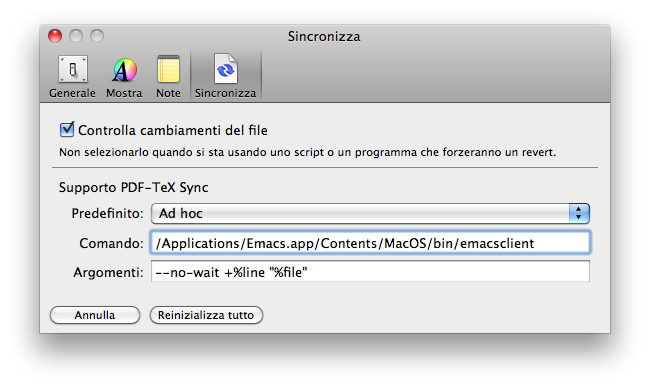
\includegraphics[width=\textwidth]{preferenze-Skim}
  \caption{Preferenze di Skim per la ricerca diretta e inversa}
  \label{fig:skimpref}
\end{figure}

La prima opzione fa sì che quando un file aperto in Skim viene
modificato da un altro processo Skim chieda se deve essere ricaricato,
scegliendo Automatico successivi aggiornamenti vengono ricaricati
senza chiedere conferma.

La configurazione di \emacs{} è analoga a quella degli altri sistemi
operativi, occorre scrivere queste righe in \emph{.emacs}
\begin{Verbatim}
(setq TeX-source-correlate-method 'synctex)
(setq TeX-source-correlate-mode t)
(setq TeX-source-correlate-start-server t)
\end{Verbatim}

Per passare dal file .tex al .pdf si utilizza la combinazione di tasti
\verb!C-c C-v!, per ritornare al file .tex bisogna fare click sulla
parola che interessa tendendo premuto shift e cmd.

Con alcune versioni di \emacs{} precedenti alla 23.3 resta in primo
piano la finestra del visulizzatore, in tal caso è necessario
aggiungere queste righe al file \emph{.emacs}
\begin{Verbatim}
(defun ns-raise-emacs ()
  (ns-do-applescript "tell application \"Emacs\" to activate"))
(add-hook 'server-switch-hook 'ns-raise-emacs)
\end{Verbatim}

\section{Skeleton mode}
\label{sec:skelmode}

\subsection{Introduzione}
\label{skelintro}

La \emph{skeleton mode} è uno speciale (ma potente) minilinguaggio,
scritto in Elisp (un dialetto di Lisp) ed incluso di default in
\emacs. Maggiori informazioni si possono ottenere digitando
\verb!C-h i d m Autotype! in \emacs.

La \emph{skeleton mode} permette in maniera molto semplice di crearsi
dei blocchi di codice (che magari si usano spesso) e di associare a
questi una combinazione di tasti per richiamarli nel proprio
documento.

Ad un livello successivo, si può anche usare questo linguaggio per
creare dei veri e propri \emph{templates}. Lo vedremo più avanti.

Per semplicità, per mostrarne l'uso, vengono di seguito riportati
degli esempi presi da una discussione sul forum del GuIT %% Il simbolo
                                %% del pacchetto da dei warning

I codici si
commentano quasi da soli:
\begin{Verbatim}
(define-skeleton TeX-dollar-sign-skeleton "Make a pair of dollar
  signs and leave point inside" nil "$"_"$" )

(global-set-key (kbd "C-x e") 'Tex-dollar-sign-skeleton)

(define-skeleton TeX-square-skeleton "Make a pair of square brackets
  and leave point inside" nil "\\[" \n _\n "\\]" )

(global-set-key (kbd "C-x s") 'TeX-square-skeleton
\end{Verbatim}
Nella prima riga si dichiara lo \emph{scheletro} con un nome, che
verrà poi utilizzato per poterlo richiamare nel codice. Segue quindi
una breve descrizione (facoltativa ma consigliata), e poi il codice
vero e proprio. Infine con \verb!global-set-key! viene creata una
combinazione di tasti personali per richiamare lo \emph{scheletro}.

Gli esempi appena mostrati sono veramente semplici e forse se ne
potrebbe fare a meno, ma servono per far capire con quanta semplicità
si possono \emph{automatizzare} certe operazioni.

\subsection{Templates}
\label{sec:skeltempl}

Talvoltà può capitare di dover scrivere documenti che hanno una forma
molto simile tra loro, o che, all'opposto, utilizziamo così raramente
che averne un modello \emph{pronto uso} risulterebbe davvero comodo.

Ecco che allora ci viene in mente di creare un file, un \emph{modello
  di documento} già configurato, da richiamare nel nostro editor
preferito.

Per \emacs{} esistono diversi pacchetti che consentono di creare
\emph{template}, ognuno dei quali richiede una installazione. Per fare
questo possiamo invece avvalerci anche della \emph{skeleton mode}
inclusa già in \emacs{}.

Supponiamo di voler creare un \emph{modello di lettera} da usare
velocemente all'occorrenza. Lo \emph{scheletro} di codice che verrà
incluso nel documento va appunto nel file \emph{.emacs}. Un prototipo
semplice potrebbe essere il seguente:

\begin{Verbatim}
(define-skeleton LaTeX-skeleton-letter "Inserts a Latex letter
skeleton into current buffer.  This only makes sense for empty
buffers."  "Destinatario: "
"\\documentclass[a4paper,10pt]{letter}\n"
"\\usepackage[T1]{fontenc}\n"
"\\usepackage[utf8]{inputenc}\n"
"\\usepackage[italian]{babel}\n"
"\\name{Pinco Pallino}\n"
"\\address{Via Marco Polo 32\\\\ Napoli 80100\\\\ Italy}\n"
"\\begin{document}\n"
"\\begin{letter}{" str | " *** Destinatario  *** " "}\n"
"\\opening{" _ "}\n\n"
"\\closing{Cordialmente}\n"
"\\end{letter}\n"
"\\end{document}\n")
\end{Verbatim}

Come già detto dopo aver dichiarato il nome dello \emph{scheletro}
seguono una o due (o a piacere) righe di commento. La riga:
\begin{Verbatim}
"Destinatario: "
\end{Verbatim}
è una riga di prompt che userà il \emph{minibuffer} per interagire con
l'utente quando verrà letto (o trovato) il simbolo \verb!str! nel
codice; il valore inserito dall'utente verrà proprio sostituito a
\verb!str!.

Il simbolo '\_' indica la posizione dove verrà posto il cursore quando
il codice \emph{skeleton} è completamente inserito.

Il codice che si vuole inserire va sempre tra due doppi apici, i
comandi vanno preceduti da un \emph{backslash} e per ritornare a capo
si usa \verb!\n!.

Infine, come precedentemente detto, si può richiamare il \emph{codice
  pronto uso} con una combinazione di tasti personale, ad esempio se
si vuole usare la combinazione \verb!C-c l!, bisogna scrivere nel file
\emph{.emacs}:
\begin{Verbatim}
(global-set-key "\C-cl" 'LaTeX-skeleton-letter)
\end{Verbatim}

Ulteriori approfondimenti (oltre a quelli a cui si perviene con
\verb!C-h i d m Autotype!) si possono reperire on-line alla pagina di
riferimento (
\href{http://www.emacswiki.org/emacs/SkeletonMode}{Skeleton Mode}).

\section{Reference Card}
\label{sec:refcard}

Oltre alla vasta documentazione che si può reperire in rete ed ai
manuali ufficiali, di particolare utilità sono le \emph{Reference
  Card}, disponibili sia per \emacs{}, sia per \auctex{}.

Si tratta di un elenco delle principali funzionalità e dei comandi a
queste associate per poter, all'occorrenza, ricordare e trovare
velocemente quello che serve.

Il tutto è riportato in maniera ordinata e concisa in una sorta di
forma tabulare, eventualmente da stampare, e tenere a portata di mano
sulla propria scrivania.

Le reference card sono disponibili sia in rete, sia sul proprio
computer una volta installati \emacs{} ed \auctex. Sul proprio
computer dovrebbero esserci anche i sorgenti pronti per essere
compilati.

\begin{figure}[t]
 \centering
 \unitlength=0.005\textwidth
 \begin{picture}(200,120)
  \put(0,0){\framebox(94,120){%
   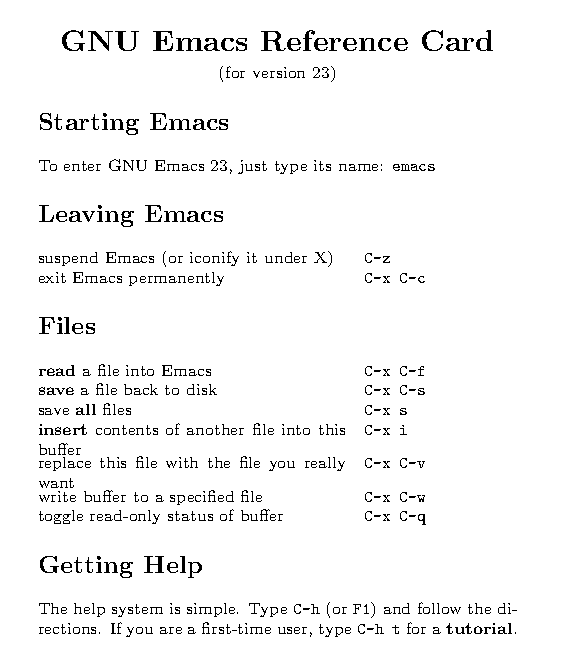
\includegraphics[width=0.51\textwidth]{refemacs}}}
  \put(95,0){\rotatebox{90}{\tiny Immagine estratta da
   \href{http://www.ps.uni-saarland.de/courses/prog-ws10/downloads/emacs_re
     fcard.pdf}{GNU Emacs Reference Card}}}
  \put(100,0){\framebox(94,120){%
   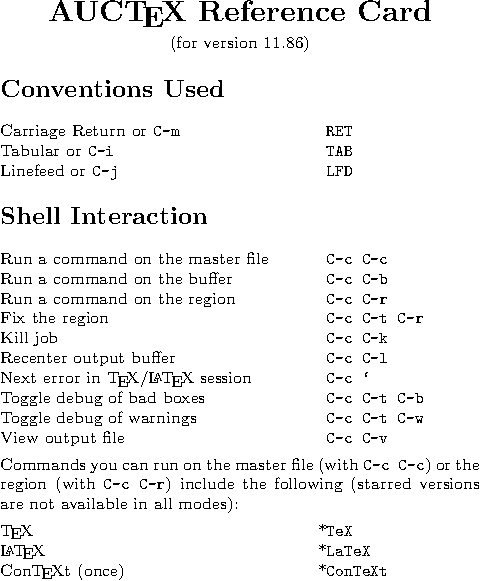
\includegraphics[width=0.51\textwidth]{refauctex}}}
  \put(195,0){\rotatebox{90}{\tiny Immagine estratta da
   \href{http://devcheatsheet.com/static/pdf/auctex-ref.pdf}{AUC\TeX{}
     Reference Card}}}
  \end{picture}
\end{figure}

\section{Conclusioni}
\label{sec:fine}

\textcolor{red}{\lipsum[1]}

\clearpage
\phantomsection
\addcontentsline{toc}{section}{\bibname}
\nocite{*}
\printbibliography

\vfill
\phantomsection
\addcontentsline{toc}{section}{Licenza d'uso \& Colophon}
\section*{Licenza d'uso \& Colophon}
\label{sec:lic}

Quest'opera è soggetta alla Creative Commons Public License versione 3.0 o
posteriore: \emph{Attribuzione}, \emph{Non Commerciale}, \emph{Condividi} allo
stesso modo. L'enunciato integrale della licenza è reperibile sul sito ufficiale
(\url{http://creativecommons.org/licenses/by-nc-sa/3.0/deed.it}).\\%

\noindent La realizzazione di questo lavoro a sei mani si è resa possibile
grazie al sistema di controllo di versione Git (\url{http://git-scm.com}). Per
poter collaborare si può clonare il progetto tramite il sito Gitorius con %
\verb!git clone git://gitorious.org/emacs-tutorial/emacs-tutorial.git!. È
gradita la segnalazione di errori o refusi.
\end{document}

%%% Local Variables:
%%% mode: latex
%%% coding: utf-8
%%% TeX-master: t
%%% fill-column: 80
%%% End:

% LocalWords:  mirror OS For dmg Git Fast Version Control System clonare git
% LocalWords:  clone
